\documentclass[]{formalLabReport}

\usepackage{graphicx}

\usepackage{tikz}

%%%%%%%%%%%%%%%%%%%%%%%%%%%%%%%%%%%%%%%%%%%%%%%%%%%%%%%%%%%%%%%%%%%%%%
% LaTeX Overlay Generator - Annotated Figures v0.0.1
% Created with http://ff.cx/latex-overlay-generator/
% If this generator saves you time, consider donating 5,- EUR! :-)
%%%%%%%%%%%%%%%%%%%%%%%%%%%%%%%%%%%%%%%%%%%%%%%%%%%%%%%%%%%%%%%%%%%%%%
%\annotatedFigureBoxCustom{bottom-left}{top-right}{label}{label-position}{box-color}{label-color}{border-color}{text-color}
\newcommand*\annotatedFigureBoxCustom[8]{\draw[#5,thick,rounded corners] (#1) rectangle (#2);\node at (#4) [fill=#6,thick,shape=circle,draw=#7,inner sep=2pt,font=\sffamily,text=#8] {\textbf{#3}};}
%\annotatedFigureBox{bottom-left}{top-right}{label}{label-position}
\newcommand*\annotatedFigureBox[4]{\annotatedFigureBoxCustom{#1}{#2}{#3}{#4}{white}{white}{black}{black}}
\newcommand*\annotatedFigureText[4]{\node[draw=none, anchor=south west, text=#2, inner sep=0, text width=#3\linewidth,font=\sffamily] at (#1){#4};}
\newenvironment {annotatedFigure}[1]{\centering\begin{tikzpicture}
\node[anchor=south west,inner sep=0] (image) at (0,0) { #1};\begin{scope}[x={(image.south east)},y={(image.north west)}]}{\end{scope}\end{tikzpicture}}
%%%%%%%%%%%%%%%%%%%%%%%%%%%%%%%%%%%%%%%%%%%%%%%%%%%%%%%%%%%%%%%%%%%%%%


\graphicspath{ {./images/} }
\begin{document}

\title{Electronics Online Challenge}
\author{Andrew Kempen, Nathan DuPont}
\submissionDate{11/13/2020}

\maketitle

\tableofcontents

\newpage

\begin{figure}[h!t]

\begin{annotatedFigure}
    {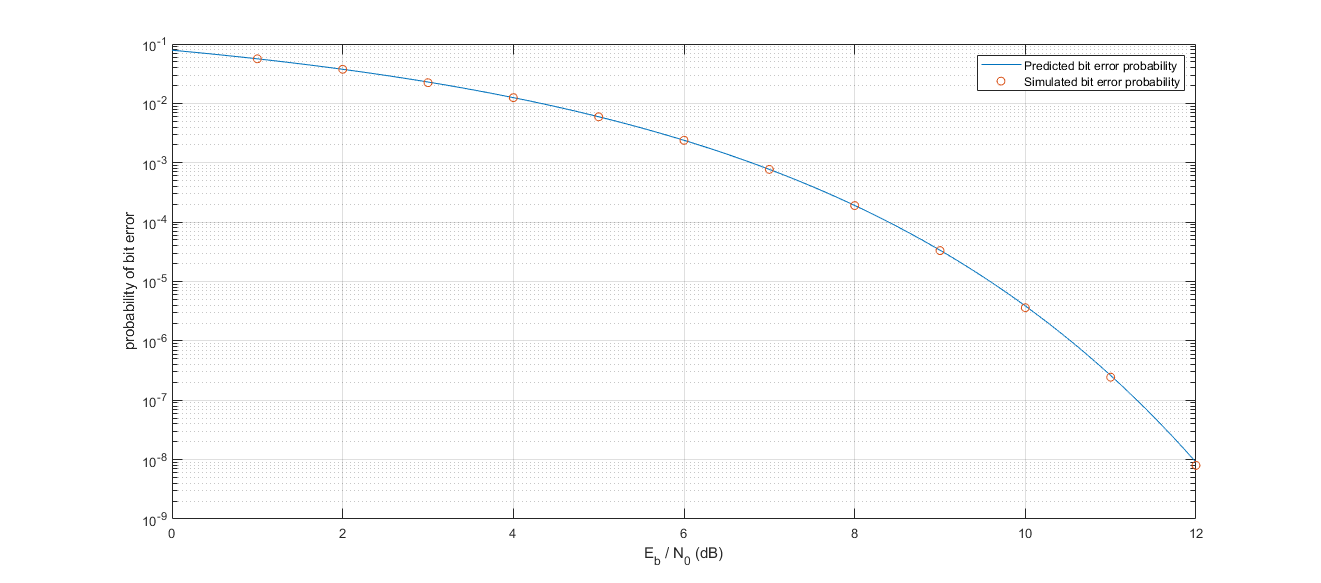
\includegraphics[width=1.0\linewidth]{report.png}}
    \annotatedFigureBox{0.176,0.5728}{0.486,0.7628}{A}{0.176,0.5728}%bl
    \annotatedFigureBox{0.32,0.19}{0.4,0.3}{B}{0.32,0.19}%bl
    \annotatedFigureBox{0.582,0.6903}{0.622,0.7803}{C}{0.582,0.6903}%bl
\end{annotatedFigure}


\caption{\textbf{Lorum Ipsum Overview} -- Lorem ipsum dolor amet (A), consetetur (B) elitr, sed diam (C) nonumy eirmod invidunt ut labore (D).}
\label{fig:teaser}

\end{figure}

\end{document}